\documentclass[tikz,border=10pt]{standalone}
% Scale s = 0.017621 cm/px, origin at O, y flipped
\begin{document}
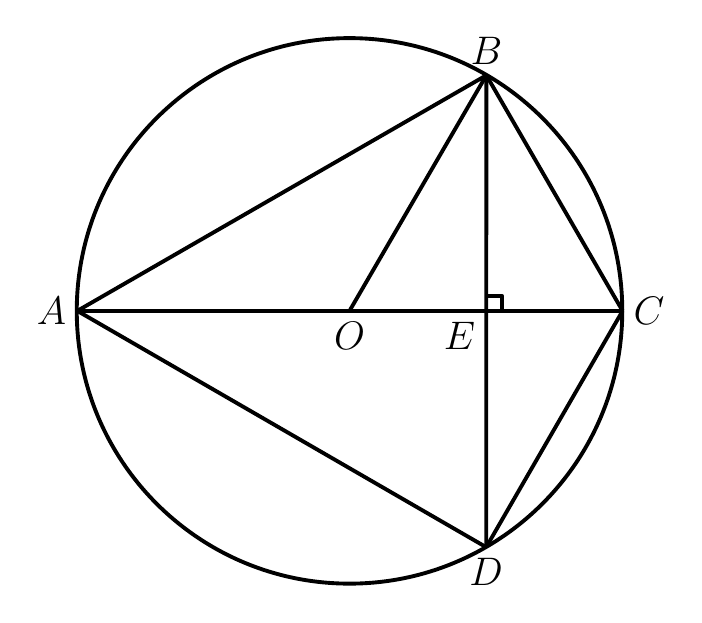
\begin{tikzpicture}[line width=1.4pt, line join=round, font=\fontsize{14.5}{17.4}\selectfont]
  % Named coordinates (converted from pixels)
  \coordinate (O) at (0,0);
  \coordinate (A) at (-3.457,0);
  \coordinate (C) at (3.468,0);
  \coordinate (E) at (1.738,0);
  \coordinate (B) at (1.738,2.992);
  \coordinate (D) at (1.736,-3.001);

  % Circle with centre O, radius 196.6 px
  \draw (O) circle[radius=3.464];

  % Segments
  \draw (A) -- (C);
  \draw (B) -- (D);
  \draw (A) -- (B);
  \draw (A) -- (D);
  \draw (B) -- (C);
  \draw (C) -- (D);
  \draw (O) -- (B);

  % Right-angle mark at E (toward C and B)
  \draw (1.738,0.194) -- (1.932,0.194) -- (1.932,0);

  % Labels
  \node[left] at (A) {$A$};
  \node[right] at (C) {$C$};
  \node[below] at (O) {$O$};
  \node[below left] at (E) {$E$};
  \node[above] at (B) {$B$};
  \node[below] at (D) {$D$};
\end{tikzpicture}
\end{document}